\documentclass{beamer}
\usetheme{AnnArbor}
\usecolortheme{beaver}
\geometry{paperwidth=140mm,paperheight=105mm}
\usepackage[utf8]{inputenc}
\usepackage[T1]{fontenc}
\usepackage[italian]{babel}
\usepackage{soul}
\usepackage{graphicx}
\usepackage{algorithm2e}
\usepackage{multirow}

\usepackage{fancyvrb}
\definecolor{felinesrcbgcolor}{rgb}{1,1,0.85}
\definecolor{felinesrcbgcolor}{rgb}{0.94,0.97,1}
\definecolor{felineframe}{rgb}{0.79,0.88,1}
\definecolor{myorange}{rgb}{1,0.375,0}
\fvset{frame=lines,
  framesep=3mm,
  framerule=3pt,
  fontsize=\small,
  rulecolor=\color{myorange},
  formatcom=\color{DarkGreen},
}

\hypersetup{
	urlcolor=myorange
}

\title[Arch2013] % (optional, only for long titles)
{Architettura degli elaboratori 2012/2013}
\subtitle{Aritmetica binaria: Signed, Fixed e Float}
\author{Michele ``Jazzinghen'' Bianchi\inst{1}}
\institute[DISI] % (optional)
{
  \inst{1}%
  Dipartimento di Ingegneria e Scienze dell'Informazione\\
  Universtià degli Studi di Trento
}
\date[2013-03-06] % (optional)
{06 Marzo 2013}
\subject{Computer Science, Embedded Systems}

\begin{document}
	\frame{\titlepage}
	\section{It's answer TIME!}
	\begin{frame}
    \frametitle{Alcune cose prima d'iniziare}
    \framesubtitle{Ve l'avevo detto che avrei risposto}
		\begin{itemize}
			\item La t-shirt che indossavo l'altra volta era di Think Geek: \url{http://www.thinkgeek.com/product/dae9/}\footnote{Quella
				di oggi è di \url{http://www.redbubble.com/}}
			\item Il mio sito web (quello con sopra la roba) è: \url{http://disi.unitn.it/~bianchi}. È fatto con
				jQuery, PHP, HTML5 e CSS3.
			\item La parte in assembly verrà fatta usando l'X86\_64.
			\item GCC bara! La somma tra uint{8,16,32,64} ed int viene fatta attraverso magheggiamenti\footnote{Dettagli sul sito}!
		\end{itemize}
	\end{frame}   
   
  \section[Being negative]{Interi con il segno}
	\subsection{Riassunto dell'ultima puntata}  
  \begin{frame}
    \frametitle{Cos'è successo l'ultima volta?}
		Abbiamo visto:    
    \begin{itemize}
    		\item Come sono stati rappresentati i numeri durante le ere
    		\item Le varie strutture dati utilizzate dai computer
    		\item Come passare da base-2 a base-10 ed il contrario
    		\item L'aritmetica con i Naturali binari
    		\item Come aggiungere il segno ai numeri binari
    \end{itemize}
    %Unari, Babilonesi, Romani, Posizioniali (indiani), Binaria
  \end{frame}
	
	\subsection{Somma / Sottrazione}
  \begin{frame}
    \frametitle{Interi con il segno}
    \framesubtitle{Somma e Sottrazione}
    Le due operazioni sono la stessa cosa!
    
		\vspace{2em}    
    
    Grazie alla convenzione usata (Complemento-2) basta sommare due numeri signed, 
    ignorando il bit di overflow, per avere il risultato.
  \end{frame}
  
  \begin{frame}
	    \frametitle{Somma e Sottrazione di interi}
	    \framesubtitle{Esempio}
	    $$117_{10} - 34_{10} = 01110101_{2} + 11011110_{2} = \text{?}$$
	    \vspace{2em}
	    \pause
			\begin{center}
			\begin{tabular}{cccccccc|c} 
			 0 & 1 & 1 & 1 & 0 & 1 & 0 & 1 & + \\  
			 1 & 1 & 0 & 1 & 1 & 1 & 1 & 0 & = \\ 
			\hline 
			 0 & 1 & 0 & 1 & 0 & 0 & 1 & 1 &  \\ 
			\end{tabular}
			\end{center}
			\pause
			\vspace{2em}
			$$01010011_{2} = 83_{10}$$
	  \end{frame}

	\subsection{Moltiplicazione signed}  
  \begin{frame}
    \frametitle{Moltiplicazione signed: Algoritmo di Booth}    	
		Possiamo moltiplicare i signed come facevamo con gli unsigned,
		solo che questo può richiedere una quantità di tempo impressionante.
		
		\vspace{2em}
		
		È per questo che utilizziamo un metodo creato da Andrew Donald Booth, che studiava,
		ovviamente, cristallografia.
		
		\vspace{2em}
		
		Il processo utilizza un concetto molto semplice, ovvero che:
		
		$$01\text{...}1 = 10\text{...}0 - 1$$
		
		Questo fa sì che sia molto buono con lunghe serie di 1 o 0, ma pessimo nel
		caso di \emph{burst} di 10 (o 01).
  \end{frame}
  \begin{frame}
    \frametitle{Moltiplicazione signed: Algoritmo di Booth}
    \framesubtitle{L'algoritmo di Booth}
    \begin{columns}
    \column{.5\textwidth}
    	  L'algoritmo è molto semplice.
    	  
    	  Si tratta di scorrere le cifre del secondo termine del
    	  prodotto e guardare la cifra immediatamente a destra
    	  (la prima cifra a destra è sempre 0).
    	  
			\vspace{2em}    	  
    	  
    	  In base a quale è la coppia bisognerà sommare o sottrarre
    	  il primo termine del prodotto.
    \column{.5\textwidth}
    		\begin{center}
			\begin{tabular}{|c||p{6em}|}
				\hline				
				Coppia di valori & Operazione \\
				\hline
				00 & \multirow{2}{*}{Nulla} \\
				11 & \\
				\hline				
				10 & Sottrare il moltiplicando 	\\
				\hline				
				01 & Sommare il motiplicando 		\\
				\hline 
			\end{tabular}
			\end{center}
    \end{columns}
  \end{frame}

  \begin{frame}
    \frametitle{Moltiplicazione signed: Algoritmo di Booth}
    \framesubtitle{Esempio}
    $$9_{10} * -13_{10} = 00001001_{2} * 11110011_{2} = ?$$
    \pause
    \begin{center}
    		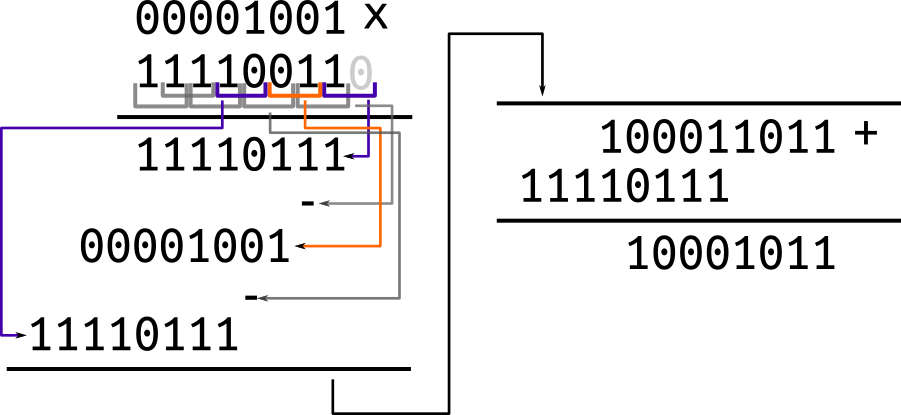
\includegraphics[width=.8\textwidth]{IMGs/Booth.png}
    \end{center}
    \pause
    \vspace{1em}
    $$10001011_{2} = -117_{10}$$
  \end{frame} 
  
  \section[Fixed]{Numeri binari frazionari}
  \begin{frame}
  		\frametitle{Un test}
  		Ok, quanto è $11101.01001_{2}$ in base-10? (solo positivo)
  		
  		\vspace{2em}
    \pause
		\begin{center}
		\begin{tabular}{ccccccccccc} 
		 $2^4$ & $2^3$ & $2^2$ & $2^1$ & $2^0$ & . & $2^{-1}$ & $2^{-2}$ & $2^{-3}$ & $2^{-4}$ & $2^{-5}$ \\		 
		 1 & 1 & 1 & 0 & 1 & . & 0 & 1 & 0 & 0 & 1 \\ 
		\hline 
		 16 & 8 & 4 & 0 & 1 & . & 0 & $1/4$ & 0 & 0 & $1/32$ \\ 
		\end{tabular}
		\end{center}
		\pause
		\vspace{2em}
		
		$$11101.01001_{2} = 29_{10} + \frac{9}{32}_{10} = 29.28125_{10} $$
  		
  \end{frame}
  \begin{frame}
  		\frametitle{Numeri binari frazionari: Fixed Point}
  		Funzionano come i numeri interi, solo che la parte a destra del "punto binario" è formata
  		da potenze frazionarie di due (i.e. potenze negative di 2).
  		
  		\vspace{2em}
  		
  	  Tutte le operazioni sono come quelle che abbiamo visto per gli interi (somma, sottrazione, moltiplicazione, shifting)
  	  
  	  \vspace{2em}
  	  
  	  \begin{block}{Utilizzo fixed Point}
  	  		Questa rappresentazione dei numeri viene utilizzata su sistemi che non dispongono di una Floating
  	  		Point Unit (FPU). Una volta erano molto più utilizzati. Tipo nella PS1, nel Saturn, nel GBA, nel
  	  		Nintendo DS... NEL SATURN! Vuol dire che il Dreamcast aveva già una FPU (anzi 4)
  	  \end{block}
    
  \end{frame}
  \subsection{Limiti}
	\begin{frame}
    \frametitle{Fixed Point}
    \framesubtitle{Limiti}
    \begin{itemize}
			\item Pochi linguaggi hanno un supporto built-in dei Fixed (C e C++ ce l'hanno grazie a GCC)
    		\item Possono rappresentare solo numeri nella forma $\frac{k}{2^x}$
    		\item Tutti gli altri numeri razionali si possono rappresentare
    			solo usando una serie di bit decimali periodica.
    \end{itemize}
    \vspace{1em}
    $$\frac{1}{3}_{10} = 0.\overline{01}_{2}$$
    $$\frac{1}{5}_{10} = 0.\overline{0011}_{2}$$
    $$\frac{1}{10}_{10} = 0.0\overline{0011}_{2}$$
  \end{frame}
  \section{Floating Point}
 	\begin{frame}
 		\frametitle{I floating points: virgole instabili}
    \framesubtitle{Intro}
    \begin{center}
    		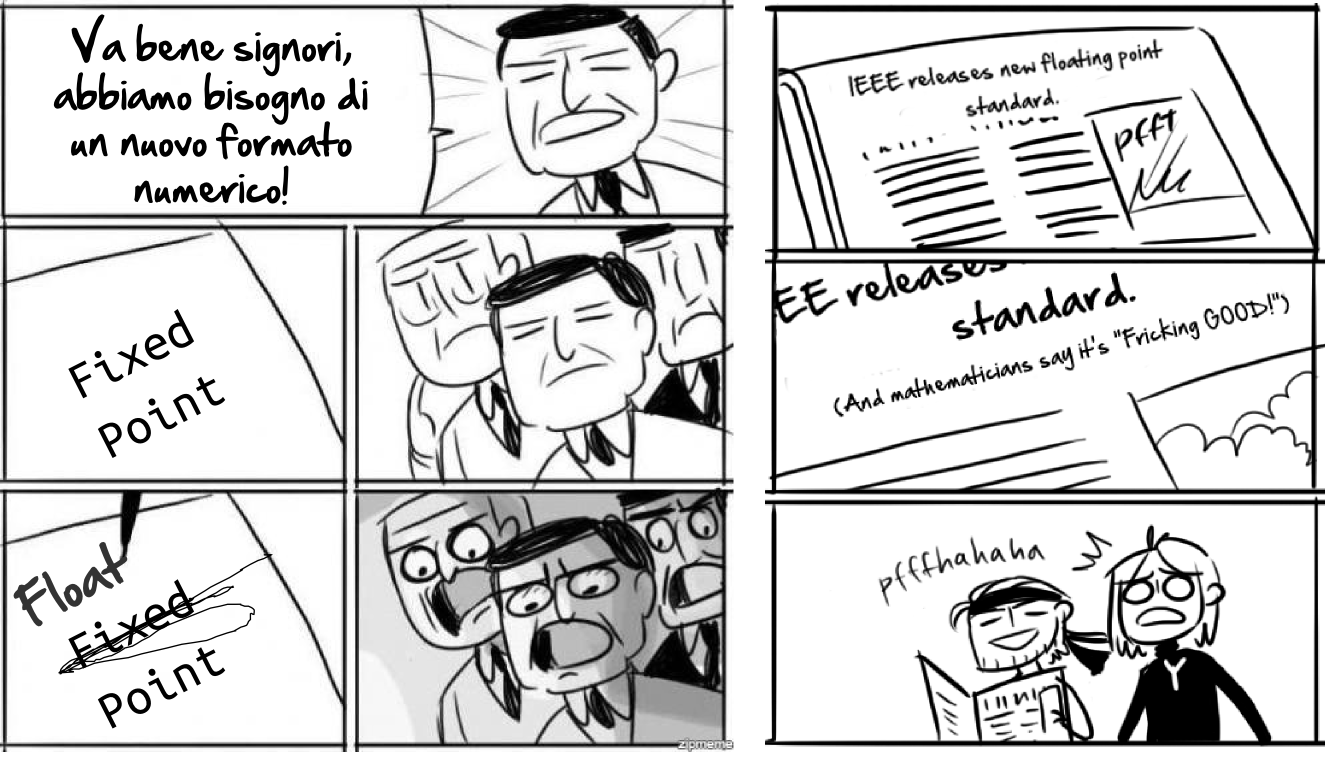
\includegraphics[width=.8\textwidth]{IMGs/MGS-FP1.png}
    \end{center}
	\end{frame} 	 
  
  \subsection{I soliti casini}
	  \begin{frame}
	    \frametitle{Floating Point: Virgole instabili}
	    \framesubtitle{Ah, buttare via i soldi}
	    È l'estate del 1994 ed il professor Nicely sta scrivendo un codice per contare
	    i numeri primi, i numeri primi gemelli, le triplette e le quadruple fino a $6.4*10^{15}$.
	    
			\vspace{2em}	    
	    
	    Questo programma ha girato per 13 anni su una ventina di PC in parallelo, però, prima
	    di iniziare i lavori seri, ha deciso di fare dei test, calcolando valori nell'ordine
	    di grandezza di $10^{13}$ e confrontandoli con dei risultati certificati, trovando delle
	    discrepanze.
	    
	  \end{frame}
	  
	  \begin{frame}
	  		\frametitle{Floating Point: Virgole instabili}
	    \framesubtitle{Ah, buttare via i soldi, Cont.}
	  	    
	    Testò il software su due macchine differenti, un Intel P6 ed un 486DX-33\footnote{Hei,
	    dovrei averne uno da qualche parte in camera!}, ed anche lì riscontrò risultati differenti
	    con ordini d'errore troppo grossi per venir generati dall'arrotondamento.
	    
			\vspace{2em}	  	    
	    
	    Dopo di questo provò di tutto: errori introdotti dal compilatore, provò a disattivare le FPU.
	    Controllò persino se non fosse il BUS PCI. Alla fine scoprì che il problema era in una serie
	    di processori Intel (le P6), testandolo anche su delle macchine in esposizione in un negozio
	    locale di informatica.
	    
	  \end{frame}
	  
	  \begin{frame}
	  		\frametitle{Floating Point: Virgole instabili}
	    \framesubtitle{Ah, buttare via i soldi: Grand Finale}
	  	    
	    Com'è andata a finire? Il Professor Nicely ha completato la sua ricerca nel 2006, utilizzando
	    486DX-33 ed altre macchine, cambiate nel tempo, mentre l'Intel, pensate un po', per un errore
	    che capitava una volta ogni nove miliardi di divisioni floating, ma che è stato gonfiato su
	    Internet (parliamo del 1994), ha perso una cosa come 450M\$ sostituendo gratis tutti i processori
	    agli utenti che lo richiedevano.
	    
	  \end{frame}
	  
	  \begin{frame}
	  		\frametitle{Floating Point: Virgole instabili}
	    \framesubtitle{Ah, buttare via i soldi: La scena dopo i titoli di coda}
	  
	  		\begin{center}
	  		...
	  		\end{center}
	  		
	  		\pause
	    
			\begin{center}
	    		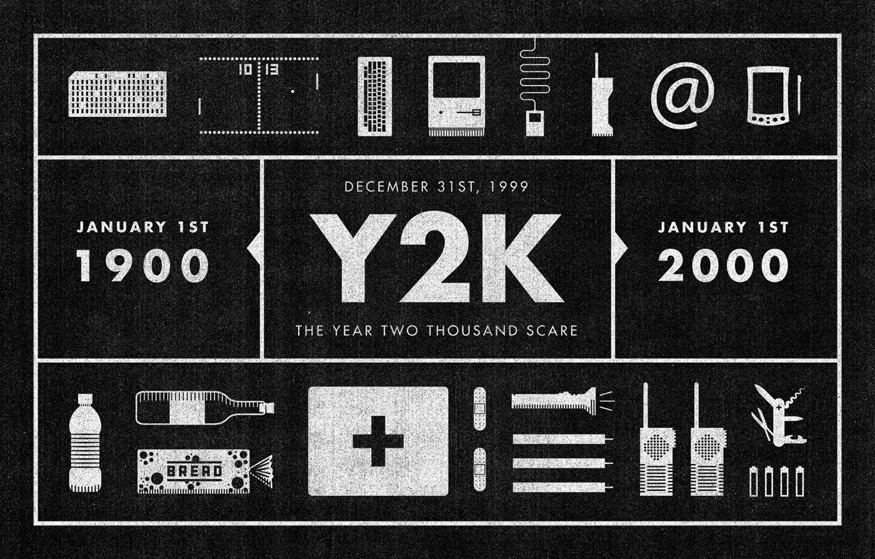
\includegraphics[width=.6\textwidth]{IMGs/Y2K.jpg}
	    \end{center}	    
	    
	    \begin{center}
	    		Mi rendo conto solo ora che questa è forse la spesa più grossa per un problema
	    		sovrastimato dopo i 300G\$ per lo Y2K.
			\end{center}	    
	    
	  \end{frame}
	  
  \subsection{Introduzione}
  \begin{frame}
    \frametitle{I floating points: virgole instabili}
    \framesubtitle{Intro cont.}
      IEEE Standard 745.
      
      \vspace{2em}
      
      È lo standard per la rappresentazione di numeri decimali con virgola mobile, ed è stato progettato
      pensando alle proprietà matematiche:
      
      \begin{itemize}
      		\item Ottimo comportamento in caso di arrotondamento, over/underflow
      		\item Il problema è che è molto complicato da implementare a livello hardware
      \end{itemize}
      
      \begin{block}{FPUs! :D}
      		In questi giorni i processori più cacciati per fare calcoli floating sono le GPU:
      		in pratica non si usano quasi gli integer per fare calcoli in 3D (da matrici di trasferimento
      		3D-2D a computazione del colore ai motori fisici)
      \end{block}
  \end{frame}
  	\subsection{Rappresentazione}
  \begin{frame}
    \frametitle{Floating Point: Virgole instabili}
    \framesubtitle{Rappresentazione dei numeri}
    I numeri floating points sono una rappresentazione in binario della notazione scientifica:
    $$(-1)^{s} * M * 2^{Exp}$$
    Dove:
    \begin{itemize}
    		\item s determina il segno del numero
    		\item M è il valore, normalmente $1.0 \leq \text{M} < 2.0$
    		\item Exp è l'esponente intero di 2 per il quale bisogna moltiplicare il tutto.
    \end{itemize}
    In forma binaria tutto questo si trasforma in:
    \begin{itemize}
    		\item 1 singolo bit s (0 positivo, 1 negativo)
    		\item una serie di bit e che indicano l'esponente
    		\item una serie di bit m che indicano la mantissa
    \end{itemize}
    E siccome c'è della simpatia nell'aria né e né m sono uguali ad M od Exp.
  \end{frame}
   
	  \begin{frame}
	    \frametitle{Floating Point: Virgole instabili}
	    \framesubtitle{Dimensioni delle componenti}
			Single:
			
			\begin{center}
				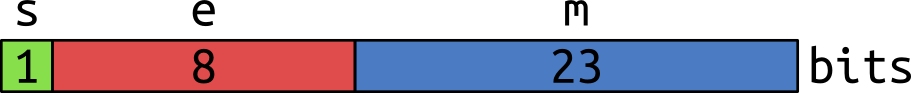
\includegraphics[width=.8\textwidth]{IMGs/Single.png}
			\end{center}
			\vspace{1em}
			Double:
			
			\begin{center}
				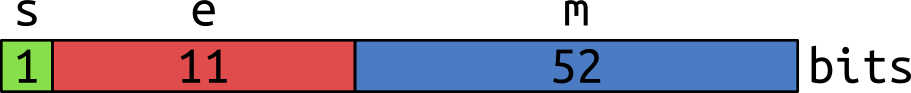
\includegraphics[width=.8\textwidth]{IMGs/Double.png}
			\end{center}
			\vspace{1em}
			Quad:
			
			\begin{center}
				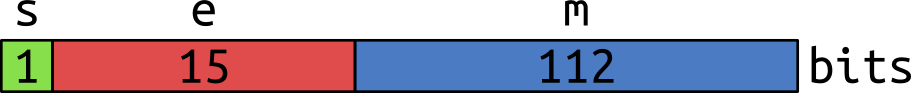
\includegraphics[width=.8\textwidth]{IMGs/Quad.png}
			\end{center}
	  \end{frame}
	  \subsection{Valori Normalizzati}
	  \begin{frame}
	    \frametitle{Floating Point: Virgole instabili}
	    \framesubtitle{Valori normalizzati}
	    Quando si ha $\text{e} \neq 0\text{...}0$ o $\text{e} \neq 1\text{...}1$ allora si ha una
	    versione normalizzata del numero in virgola mobile, ovvero:
	    
	    \begin{itemize}
	      \item Esponente (Exp): Exp = e - Bias
	      		\begin{itemize}
	      			\item Il Bias è pari a $2^{k-1} - 1$, dove k è il numero di bit dell'esponente.
	      			\item Avremmo così un range di esponenti di -126...127 per single, -1022...1023 per i double e
	      				-16383...16384 per i quad.
	      		\end{itemize}
	      \item Valore (M): $1.m_{k}m_{k-1}...m_{1}$
	      		\begin{itemize}
	      			\item Abbiamo k bit + 1 per rappresentare il valore, grazie al \emph{1.}
	      			\item Il minimo è 1.0, dato da $\text{m} = 0\text{...}0$
	      			\item Il massimo è 2.0 - $\epsilon$, dato da $\text{m} = 1\text{...}1$\footnote{$\epsilon$ è un valore
	      				piccolo a scelta. In pratica il valore M potrà arrivare a valere quasi 2, non arrivandoci mai.}
	      		\end{itemize}
	    \end{itemize}
	  \end{frame}
	  \begin{frame}
	    \frametitle{Floating Point: Virgole instabili}
	    \framesubtitle{Valori normalizzati: Esempio}
	    		$$1337.0_{10} = ?$$
	    		\vspace{1em}
	    		\pause
	    		$$1337.0_{10} = 10100111001_{2}$$
	    		Normalizziamo la mantissa: $10100111001_{2} = 1.0100111001_{2}*2^{11}$
	    	  
	    	  Mantissa: $\text{m} = 01001110010000000000000$
	    	  
	    	  Esponente:
	    	  \begin{itemize}
	    	  		\item Exp = 10
	    	  		\item Bias = 127
	    	  		\item e = Exp + Bias = 127 + 10 = 137 = $10001001_{2}$
	    	  \end{itemize}
	    	  
	    	  \vspace{1em}
	    	  \pause
	    	  \begin{center}
					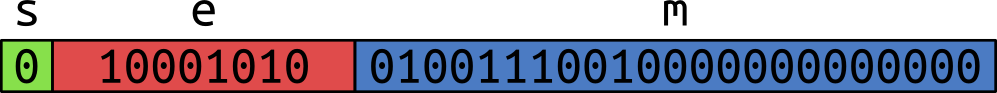
\includegraphics[width=.8\textwidth]{IMGs/SingleExample.png}
				\end{center}
	  \end{frame}
  \subsection{Valori Denormalizzati}
	  \begin{frame}
	    \frametitle{Floating Point: Virgole instabili}
	    \framesubtitle{Valori denormalizzati}
	    Quando si ha $\text{e} = 0\text{...}0$ allora stiamo lavorando con una versione
	    denormalizzata del numero in virgola mobile:
	    
	    \begin{itemize}
	      \item Esponente (Exp): Exp = -Bias + 1
	      \item Valore (M): $0.m_{k}m_{k-1}...m_{1}$, invece che $1.m_{k}m_{k-1}...m_{1}$      
	        \begin{itemize}
	      			\item Con m = 0...0, allora il float vale 0.\footnote{Così, però, avremo $+0$ e $-0$. Come mai?}
	      			\item Con $\text{m} \neq 0\text{...}0$ avremmo numeri molto piccoli vicini a 0, ma perdiamo precisione.
	      		\end{itemize}
	    \end{itemize}
	  \end{frame}
	  \subsection{Casi speciali}
	  \begin{frame}
	    \frametitle{Floating Point: Virgole instabili}
	    \framesubtitle{Casi speciali}
	    Per indicare che qualcosa è andato storto l'esponente viene settato a $\text{e} = 1\text{...}1$
	    
	    \begin{itemize}
	      \item $m = 0\text{...}0$
	      		\begin{itemize}
	      			\item Rappresenta $\infty$
	      			\item Può essere negativo o positivo
	      			\item Indica che c'è stato un overflow\footnote{Avete diviso per 0, sì?}
	      		\end{itemize}
	      	\item $m \neq 0\text{...}0$
	      		\begin{itemize}
	      			\item Rappresenta NaN
	      			\item Viene utilizzato quando non si può determinare il risultato di un'operazione, tipo $\sqrt{-1}$\footnote{per
	      				questo dovete utilizzare una libreria per i complessi} o $\infty * 0$
	      		\end{itemize}
	    \end{itemize}
	  \end{frame}
% etc
\end{document}
